%%%%%%%%%%%%%%%%%%%%%%%%%%%%%%%%%%%%%%%%%%%%%%%%%%%%%%%%%%%%%%%
%
%
%   This file is included in DeformableRegistration.tex
%
%   Labels and section entries are defined in that file.
%
%
%
%%%%%%%%%%%%%%%%%%%%%%%%%%%%%%%%%%%%%%%%%%%%%%%%%%%%%%%%%%%%%%
Let us register the deformed volumes generated by Thin plate warping in the
previous example using DeformableRegistration4.cxx. Since ITK is in general
N-dimensional, the only change in the example is to replace the
\code{ImageDimension} by 3.

The registration method uses B-splines and an LBFGS optimizer. The trace in
Table. \ref{tab:LBFGStrace} prints the trace of the optimizer through the
search space.

\begin{table}
\begin{center}
\begin{tabular}{ | p{3cm} | p{1.8cm} | p{2.5cm} | p{4cm} | }
\hline
\textbf{Iteration} &
\textbf{Function value} &
\textbf{$\|G\|$} &
\textbf{Step length} \\
\hline\hline
   1    &        156.981  &    14.911  & 0.202 \\
   2    &        68.956    &    11.774    &    1.500 \\
   3    &        38.146    &    4.802     &   1.500 \\
   4    &        26.690    &    2.515     &   1.500 \\
   5    &        23.295    &    1.106     &   1.500\\
   6    &        21.454    &    1.032     &   1.500\\
   7    &        20.322    &    1.557     &   1.500\\
   8    &        19.751    &    0.594     &   1.500\\
\hline
\end{tabular}
\end{center}
\itkcaption[LBFGS Optimizer trace]{LBFGS Optimizer trace.
\label{tab:LBFGStrace}}
\end{table}

Here $\|G\|$ is the norm of the gradient at the current estimate of the
minimum, $x$. ``Function Value" is the current value of the function, f(x).

The resulting deformation field that maps the moving to the fixed image is
shown in \ref{fig:DeformationFieldOutput}. A difference image of two slices
before and after registration is shown in
\ref{fig:DefRegistrationDiffScreenshot}. As can be seen from the figures, the
deformation field is in close agreement to the one generated from the Thin
plate spline warping.

\begin{figure}
\centering
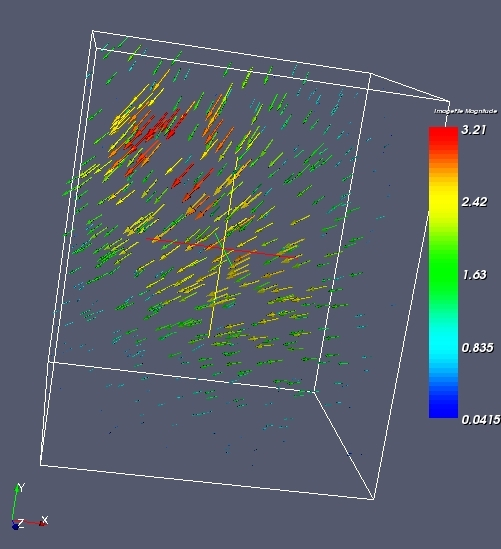
\includegraphics[width=0.6\textwidth]{ParaviewScreenshot5.eps}
\itkcaption[Deformation field output]{Resulting deformation field that maps the moving image to the fixed image.}
\label{fig:DeformationFieldOutput}
\end{figure}

\begin{figure}
\centering
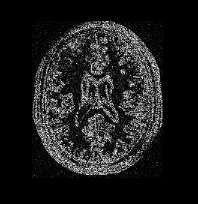
\includegraphics[width=0.44\textwidth]{DeformableRegistration4DiffBefore.eps}
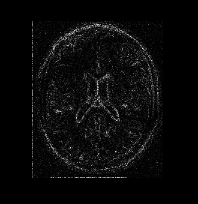
\includegraphics[width=0.44\textwidth]{DeformableRegistration4DiffAfter.eps}
\itkcaption[Difference image]{Difference image from a slice before and after registration.}
\label{fig:DefRegistrationDiffScreenshot}
\end{figure}
